\section{Interpolation-Based Compression: FDWZ}\label{sec:fdwz}

FDWZ adapts the SZ compression framework to high-order element data. Section~\ref{sec:FDWZ:sz-framework} briefly reviews its prediction--quantization pipeline. Section~\ref{sec:FDWZ:distance-weighted} introduces GLL-aware interpolation for more accurate prediction, while Section~\ref{sec:FDWZ:multi-tree} uses multi-tree Huffman encoding for more effective lossless compression, as summarized in Figure~\ref{fig:fdwz-workflow}. Finally, Sections~\ref{sec:FDWZ:cross-interface} and~\ref{sec:FDWZ:element-index-dimension} assess whether prediction across shared element interfaces or along the element-index dimension offers an advantage over element-local prediction.

\begin{figure}[htb]
    \centering
    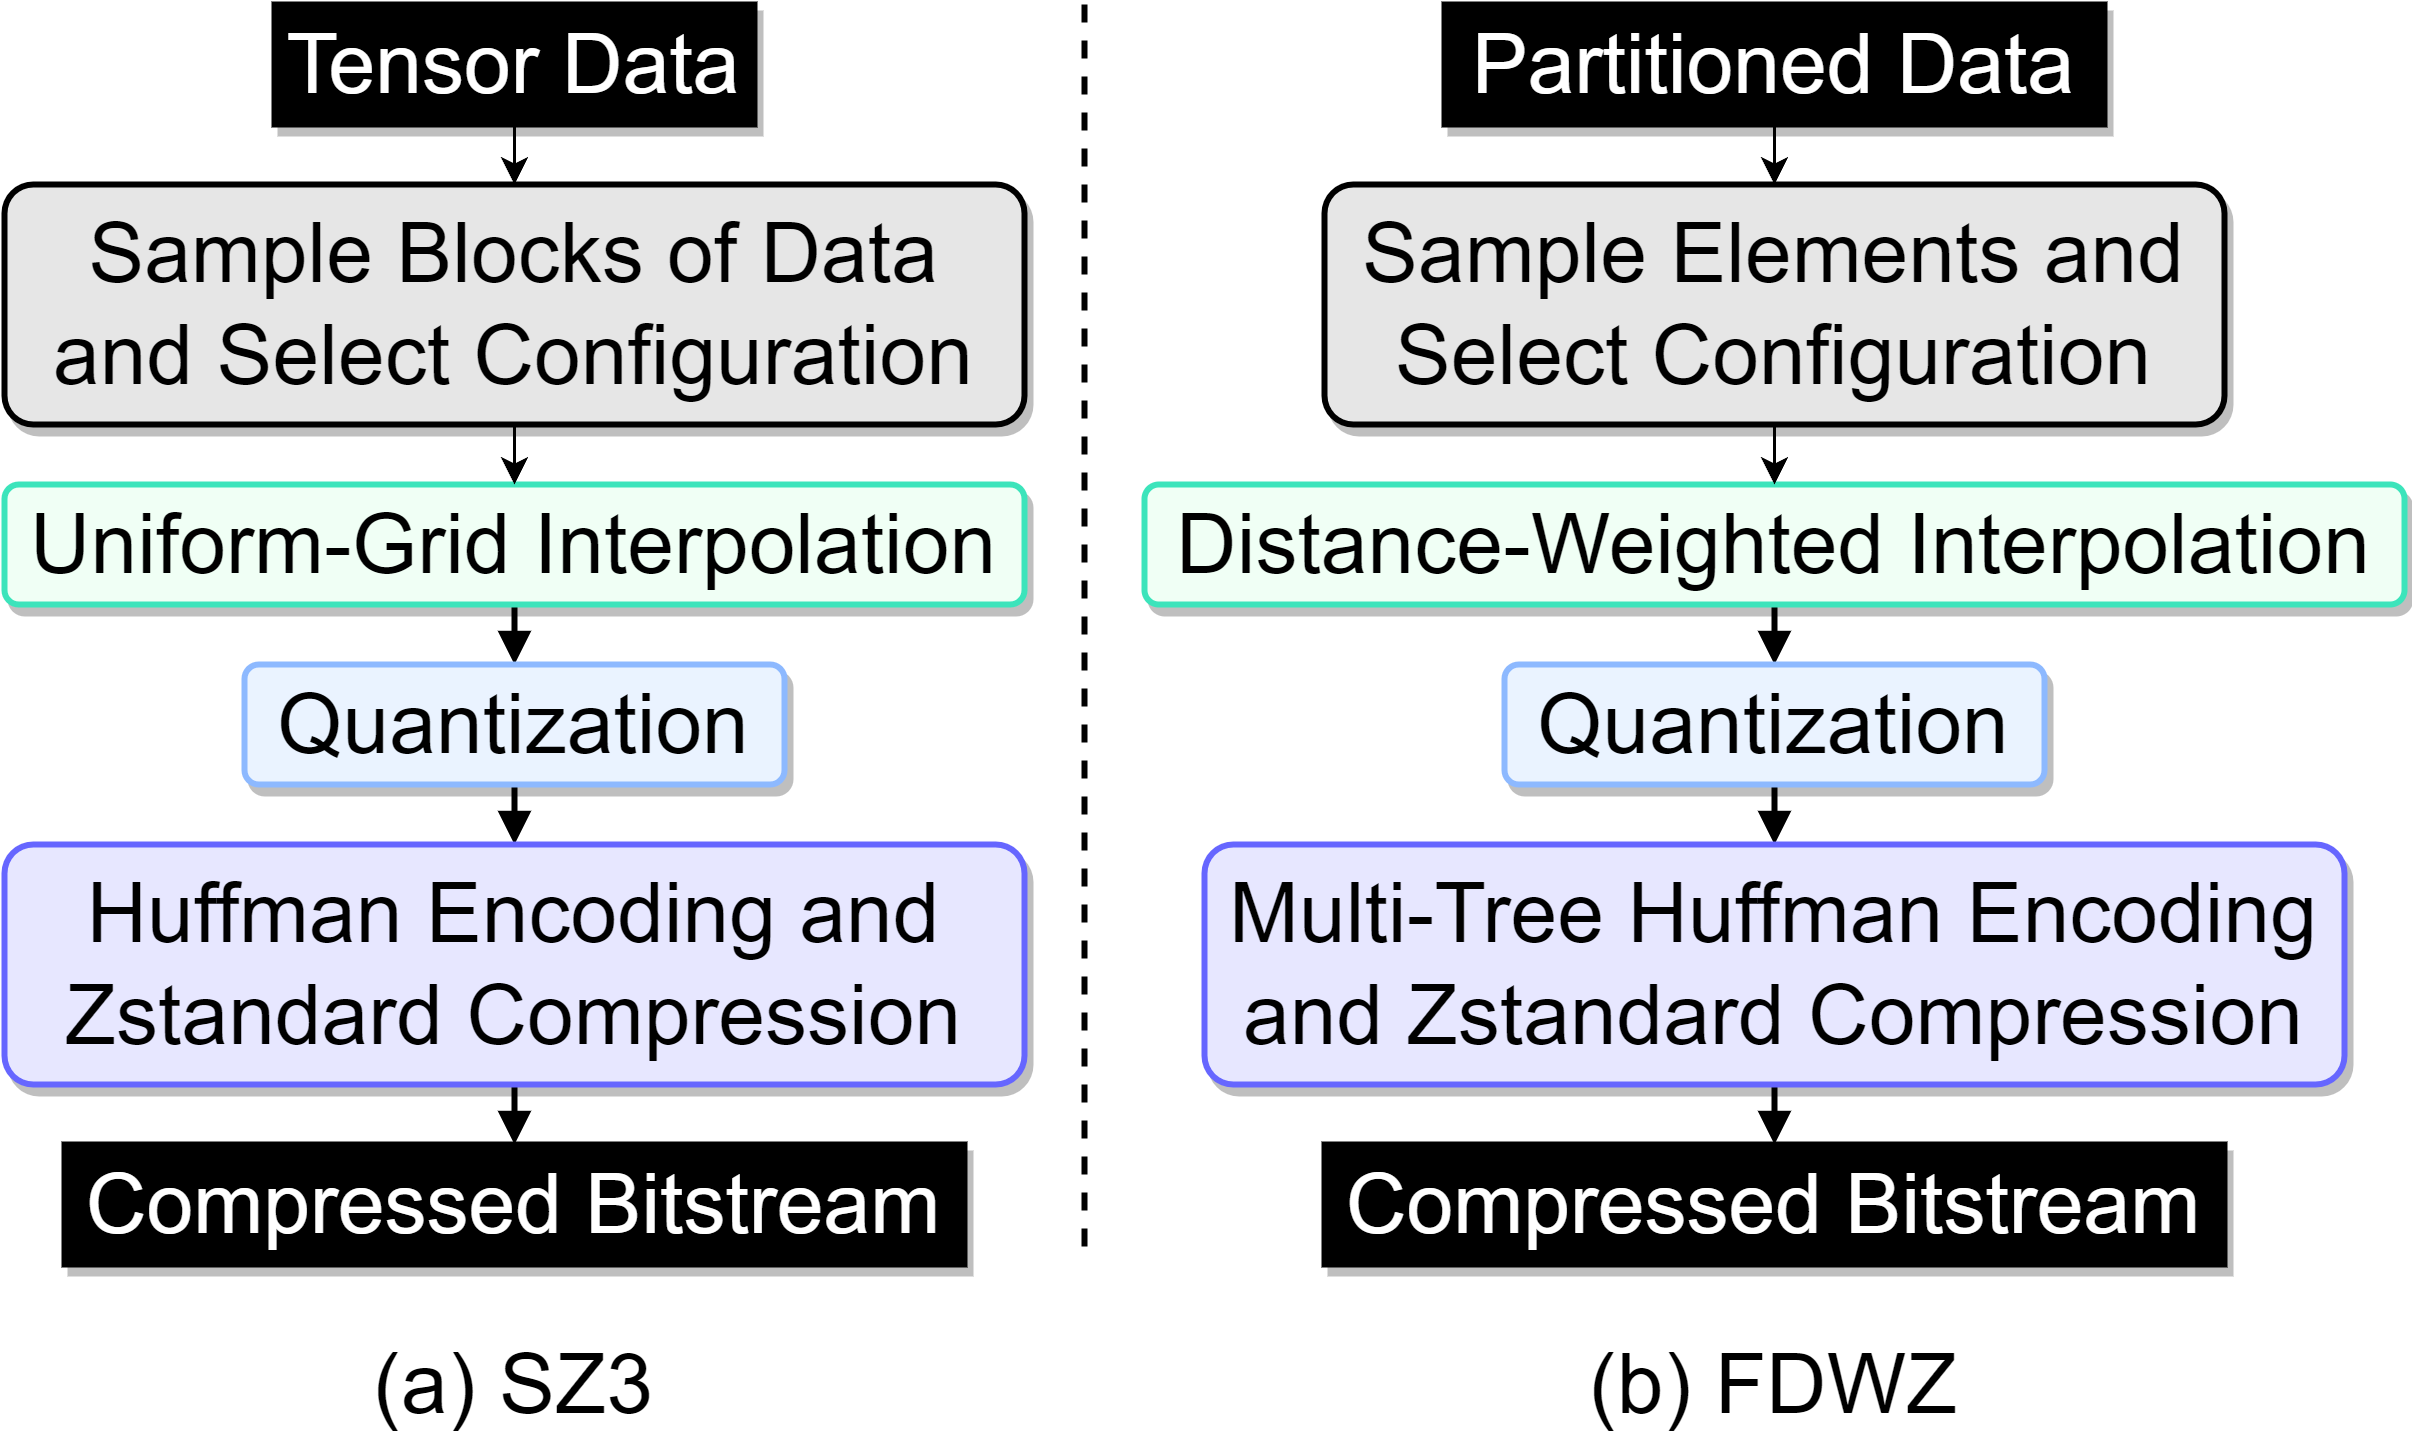
\includegraphics[width=0.9091\linewidth]{figs/5/fdwz_diagram.png}
    \caption{Comparison of standard SZ3 compression on tensor data (left) and FDWZ compression on a high-order element partition (right). FDWZ replaces uniform-grid interpolation with distance-weighted interpolation and single-tree Huffman encoding with multi-tree encoding.}
    \label{fig:fdwz-workflow}
\end{figure}

\subsection{SZ Compression Framework}\label{sec:FDWZ:sz-framework}

The SZ framework follows a prediction--quantization--encoding pipeline~\cite{tao2017significantly,liang2023sz3}. For each target value, it predicts from previously reconstructed values and quantizes the prediction error under a user-specified error bound. Using reconstructed references keeps the compressor and decompressor synchronized while preserving the pointwise error guarantee. The resulting quantization symbols are encoded using a single Huffman tree followed by Zstandard~\cite{ycollet2021zstd}. Within this pipeline, SZ3 applies multilevel interpolation to a multidimensional array, predicting points level by level.

A representative predictor in SZ3 uses cubic interpolation on a uniform array grid. As illustrated in Figure~\ref{fig:cubic-interpolation}(a), it predicts a target by evaluating the cubic polynomial fitted through four reconstructed reference values. On a uniform grid, this yields the fixed Lagrange interpolation weights listed in Table~\ref{tab:cubic-interpolation}.

\subsection{Distance-Weighted Multilevel Interpolation}\label{sec:FDWZ:distance-weighted}

FDWZ adapts this cubic interpolation to the nonuniform spacing of GLL points within each high-order element. This adaptation involves two changes: distance-weighted interpolation and a modified prediction order.

\begin{enumerate}
\item \textit{Distance-Weighted Interpolation}: Because GLL points are nonuniformly spaced, the fixed coefficients used by SZ3 no longer represent the cubic interpolant at the target position. In principle, FDWZ could compute interpolation weights from the physical coordinates of each element. However, repeating this calculation for every target in every element would be expensive. FDWZ therefore computes cubic Lagrange weights from the reference-space coordinates of the target and reference points. Figure~\ref{fig:cubic-interpolation}(b) illustrates such a stencil, and Table~\ref{tab:cubic-interpolation} lists its coordinates and weights. Because the reference-space GLL nodes depend only on the polynomial order, the resulting interpolation weights can be reused across all elements of that order.
\item \textit{Modified Prediction Order}: SZ3 constructs its multilevel hierarchy by repeatedly selecting the array-index midpoint between two reconstructed endpoints. On a uniform grid, this point is also their geometric midpoint. FDWZ instead selects the unpredicted GLL point closest to the midpoint of the two endpoints in reference space. This choice helps limit the propagation of compression errors to later prediction levels. This order is also computed once per polynomial order and reused across elements.
\end{enumerate}

For a controlled ablation, we use 7P---the $P$ field of Dataset~7 listed in Table~\ref{tab:datasets}---and compare the three predictor configurations at matched PSNRs. Replacing SZ3's uniform-grid weights with GLL weights improves the compression ratio by 62.7\% on average. With the GLL weights fixed, the modified prediction order provides a further 6.8\% average improvement.

\begin{figure}[htb]
    \centering
    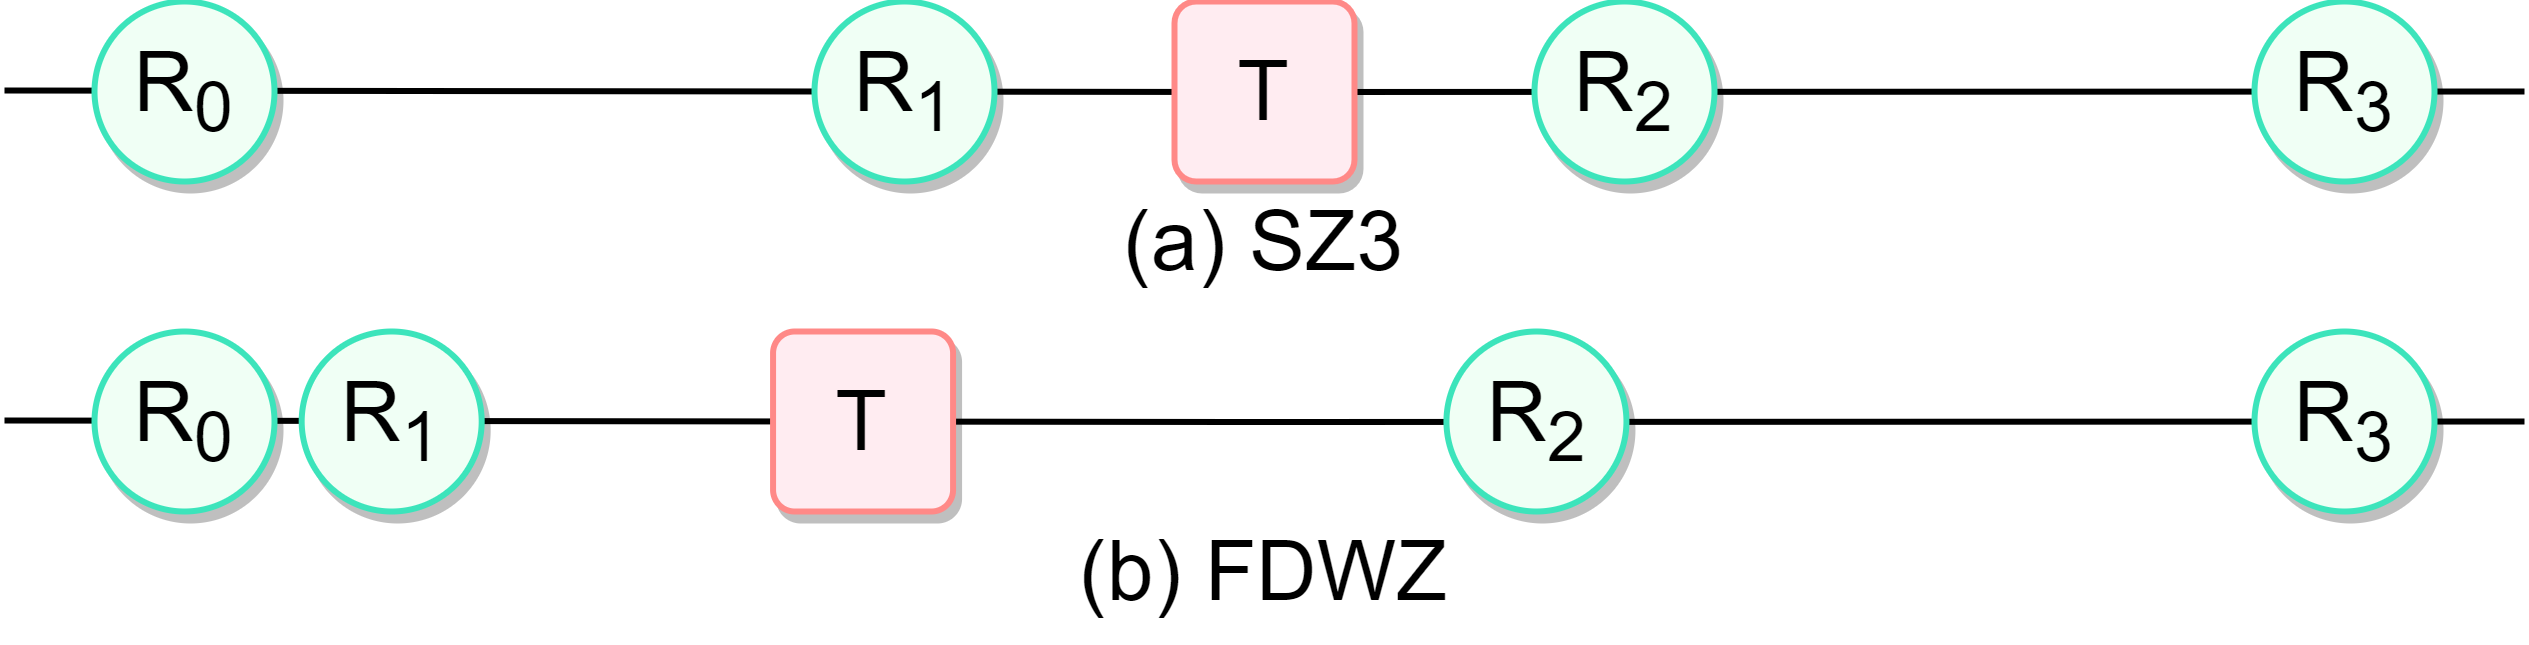
\includegraphics[width=0.9545\linewidth]{figs/5/cubic_interpolation.png}
    \caption{Comparison of cubic interpolation stencils in SZ3 and FDWZ. The distribution of GLL points within an element differs substantially from a uniform grid, producing different interpolation weights. The coordinates and weights are reported in Table~\ref{tab:cubic-interpolation}.}
    \label{fig:cubic-interpolation}
\end{figure}

\begin{table}[htb]
    \caption{Coordinates and cubic interpolation weights for the 10-point GLL example in Figure~\ref{fig:cubic-interpolation}. Here, $d$ is the spacing between adjacent points on the uniform SZ3 grid, whereas $a$ is the reference-element length along the interpolation direction.}
    \label{tab:cubic-interpolation}
    \centering
    \footnotesize
    \setlength{\tabcolsep}{2.5pt}
    \renewcommand{\arraystretch}{1.05}
    \begin{tabular*}{\columnwidth}{@{\extracolsep{\fill}}lccccc@{}}
        \toprule
        & $R_0$ & $R_1$ & $T$ & $R_2$ & $R_3$ \\
        \midrule
        SZ3: $x/d$ & \textminus3 & \textminus1 & 0 & 1 & 3 \\
        SZ3: $w$ & \textminus0.0625 & 0.5625 & --- & 0.5625 & \textminus0.0625 \\
        FDWZ: $x/a$ & 0 & 0.040 & 0.131 & 0.261 & 0.417 \\
        FDWZ: $w$ & \textminus0.771 & 1.458 & --- & 0.376 & \textminus0.063 \\
        \bottomrule
    \end{tabular*}
\end{table}

Element-local prediction also provides favorable memory locality. On large regular tensor datasets, SZ3 may perform long-range accesses during multilevel prediction, which can increase cache misses. However, the elements evaluated in this work contain at most 1,000 values, allowing FDWZ to operate primarily on cache-resident data.

\subsection{Multi-tree Huffman Encoding}\label{sec:FDWZ:multi-tree}

Quantization-symbol distributions differ across FDWZ prediction levels. Earlier levels generally use reference points farther from their targets, producing larger prediction errors and a wider distribution of quantization symbols. Later levels use closer reference points and therefore tend to produce smaller errors and symbols that are more concentrated near zero.

Encoding symbols from all levels with one Huffman tree mixes these distributions and yields code lengths that are poorly matched to individual groups. FDWZ instead assigns different prediction levels to separate Huffman trees, using at most five trees to limit codebook metadata. The encoded streams are finally compressed together using Zstandard.

Figure~\ref{fig:fdwz-tree-ablation}(a) compares prediction-error distributions across the groups of predicted values, while Figure~\ref{fig:fdwz-tree-ablation}(b) shows how the bit rate changes as the number of Huffman trees increases.

\begin{figure}[htb]
    \centering
    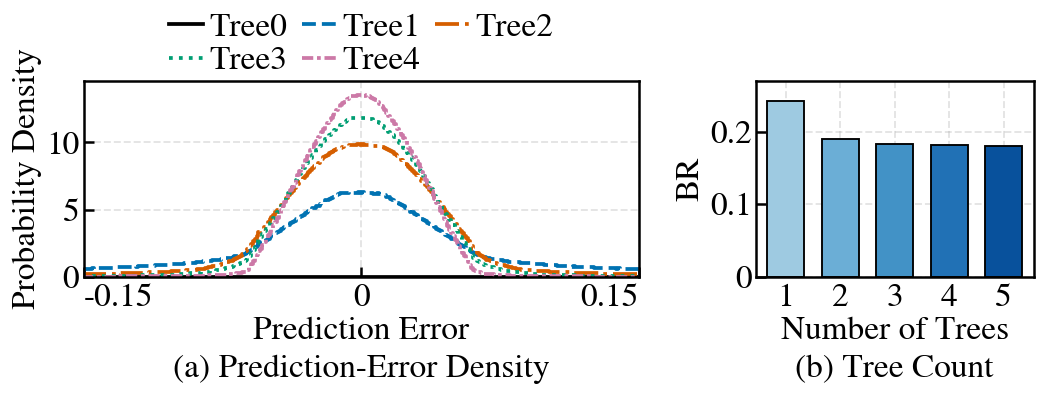
\includegraphics[width=\linewidth]{figs/5/fdwz-tree-ablation.png}
    \caption{Prediction-error distributions and tree-count ablation on 7P. (a) Raw prediction-error densities at $\varepsilon_{\mathrm{rel}}=10^{-3}$. From Tree0 to Tree4, an increasing fraction of errors concentrates near zero. Tree0 uses zero as its predictor, so its errors span a much wider range that is not visible at this scale. (b) BR at $\varepsilon_{\mathrm{rel}}=10^{-3}$ for one to five Huffman trees. Five trees improve the compression ratio over one tree by 35.1\% at this error bound and by 26.6\% on average across all five bounds.}
    \label{fig:fdwz-tree-ablation}
\end{figure}

\subsection{Prediction Across Shared Element Interfaces}\label{sec:FDWZ:cross-interface}

We next examine whether cross-interface prediction can improve upon the element-local interpolation used by FDWZ. For a controlled comparison, both predictors are evaluated at the same target points on faces shared by adjacent elements. As illustrated in Figure~\ref{fig:cross-element}, the cross-interface predictor uses two interior reference points from each adjacent element, whereas the element-local predictor uses four reference points along either reference-space direction of the shared face.

\begin{figure}[htb]
    \centering
    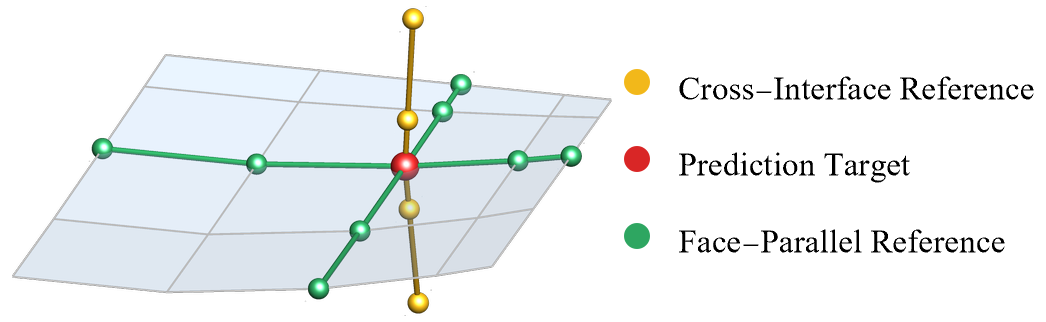
\includegraphics[width=1\linewidth]{figs/raster300/cross-element.png}
    \caption{Cubic prediction stencils across and along a shared element interface. The blue surface denotes the shared interface. The regions above and below it belong to the two adjacent elements.}
    \label{fig:cross-element}
\end{figure}

In principle, the clustering of GLL points near element boundaries allows cross-interface prediction to use reference points close to the target. However, the two elements can be geometrically distorted in different ways, and the deformation on one side need not continue smoothly onto the other. Consequently, the cross-interface reference points are generally not collinear with the target in physical space. In contrast, each face-parallel stencil lies along a tensor-product coordinate line in reference space. These competing effects make their relative prediction accuracy unclear a priori.

We therefore evaluate 7P on randomly selected internal faces, each shared by two elements, and compare the prediction errors at the same interior points of each face.

\begin{table}[htb]
    \centering
    \caption{Comparison of face-parallel and cross-interface prediction errors on internal faces in 7P. \textbf{Face-parallel} is the method used by FDWZ. The entropy column uses $\varepsilon_{\mathrm{rel}}=10^{-4}$.}
    \label{tab:cross-interface-prediction}
    \footnotesize
    \setlength{\tabcolsep}{3pt}
    \begin{tabular*}{\columnwidth}{@{\extracolsep{\fill}}lccc@{}}
        \toprule
        Method & NRMSE & NMAE & Entropy \\
        \midrule
        \textbf{Face-parallel} & $4.215\times10^{-5}$ & $8.584\times10^{-6}$ & $0.149$ \\
        Cross-interface & $5.234\times10^{-5}$ & $1.875\times10^{-5}$ & $0.398$ \\
        \bottomrule
    \end{tabular*}
\end{table}

Table~\ref{tab:cross-interface-prediction} shows that face-parallel prediction has lower NRMSE and NMAE, while cross-interface prediction produces quantized errors with 2.67$\times$ the entropy. Thus, the shorter reference distances enabled by GLL clustering do not compensate for geometric misalignment across elements. Cross-interface prediction also requires mesh connectivity and consistent face orientations. We therefore retain element-local prediction in FDWZ.

\subsection{Prediction Along the Element-Index Dimension}\label{sec:FDWZ:element-index-dimension}

We next examine whether prediction along the element-index dimension can outperform the element-local distance-weighted interpolation used by FDWZ. Section~\ref{sec:problem formulation:data characteristics} represents each scalar field as the four-dimensional logical array $X=\{x_{e,i,j,k}\}$, where $e$ enumerates the stored elements and $(i,j,k)$ identifies an element-local position. FDWZ does not exploit predictability along the dimension indexed by $e$.

We evaluate 7P, applying both methods to the same target values. The element-local method uses FDWZ's distance-weighted interpolation, while the element-index method follows QoZ's one-dimensional interpolation approach~\cite{liu2024high}. To assess the contribution of the stored element order, we also try element-index prediction after shuffling elements within each partition.

\begin{table}[htb]
    \centering
    \caption{Element-local and element-index prediction errors on 7P. \textbf{Element-local} is used by FDWZ. Shuffled element-index uses a fixed random permutation within each partition. Entropy uses $\varepsilon_{\mathrm{rel}}=10^{-4}$.}
    \label{tab:element-index-prediction}
    \footnotesize
    \setlength{\tabcolsep}{2.4pt}
    \begin{tabular*}{\columnwidth}{@{\extracolsep{\fill}}lccc@{}}
        \toprule
        Method & NRMSE & NMAE & Entropy \\
        \midrule
        \textbf{Element-local} & $3.323\times10^{-4}$ & $3.462\times10^{-5}$ & $0.511$ \\
        Element-index & $1.106\times10^{-2}$ & $4.362\times10^{-3}$ & $6.306$ \\
        Shuffled & $1.045\times10^{-1}$ & $8.036\times10^{-2}$ & $11.060$ \\
        \bottomrule
    \end{tabular*}
\end{table}

Table~\ref{tab:element-index-prediction} shows that element-index prediction produces 33.3$\times$ the NRMSE, 126$\times$ the NMAE, and 12.3$\times$ the quantized-error entropy of element-local prediction. Shuffling the elements further increases all three metrics, showing that the stored order nevertheless retains some statistical locality.
